%%
%% =====================================================================
%%  elsarticle 结构骨架
%% =====================================================================
%%  ⚠️  这不是 Elsevier 官方模板原件，而是按 elsarticle.cls 的**必需结构**
%%      写成的骨架，用途有两个：
%%        1. 作者手头没有下载官方模板时，也能生成结构正确、可直接编译的稿件；
%%        2. 作为「模板模式」的最小可用示例。
%%
%%      投正式期刊前，请用你从 Elsevier 官网下载的模板主文件替换它：
%%        python scripts/sci.py run 你的稿件 --journal elsevier-generic \
%%               --template /path/to/elsarticle-template-num.tex
%% =====================================================================
%%
\documentclass[preprint,12pt]{elsarticle}

\usepackage{amsmath}
\usepackage{amssymb}
\usepackage{graphicx}
\usepackage{booktabs}

\journal{[待作者填写：目标期刊名]}
% [sci-trans] 以下导言区命令来自原稿：模板未提供，但正文依赖它们
\usepackage{siunitx}
\usepackage{hyperref}
\usepackage[numbers,sort&compress]{natbib}
\usepackage{caption}
\usepackage{subcaption}
\usepackage{lineno}
\newcommand{\method}{Adaptive Spectral Truncation (AST)}
\DeclareMathOperator*{\argmin}{arg\,min}
\graphicspath{{figures/}}

\begin{document}

\begin{frontmatter}
\title{Adaptive Spectral Truncation for Low-Power Edge Inference of Convolutional Networks}

% [sci-trans] 模板示例作者/单位命令（保留备查）：
% \author[aff1]{Template Author}
% \ead{template.author@example.com}
% \affiliation[aff1]{organization={Template Institution}, city={City}, country={Country}}
% [sci-trans] 按目标模板命令体系重新生成的作者/单位：
\affiliation[aff1]{School of Automation, Harbin Institute of Technology, Harbin 150001, China}
\affiliation[aff2]{Peng Cheng Laboratory, Shenzhen 518055, China}
\affiliation[aff3]{Department of Electrical Engineering, University of Melbourne, Parkville, VIC 3010, Australia}
\author[aff1]{Wei Zhang}
\author[aff1,aff2]{Li Chen}
\author[aff3]{Marcus Hale}

\begin{abstract}
Background: Deploying convolutional neural networks on battery-powered edge devices is
limited by the energy cost of dense matrix multiplication.
Methods: We introduce \method{}, which estimates the spectral decay of each layer's
weight matrix at calibration time and truncates the trailing singular subspace.
Results: On CIFAR-10 and ImageNet-100 subsets, AST reduces multiply--accumulate operations
by 41.7\% while losing 0.6 percentage points of top-1 accuracy.
Conclusions: AST is complementary to quantization and can be stacked with 8-bit
post-training quantization for an additional 1.9$\times$ energy reduction.
\end{abstract}

\begin{keyword}
edge inference \sep model compression \sep spectral methods \sep convolutional neural networks \sep energy efficiency
\end{keyword}
\end{frontmatter}

\section{Introduction}
\label{sec:intro}

Convolutional neural networks (CNNs) have become the default architecture for
perception on embedded platforms \citep{lecun2015deep,he2016deep}. However, the
energy budget of a battery-powered node is dominated by the multiply--accumulate
(MAC) operations of dense convolutions \citep{horowitz2014computing}.

Prior work reduces this cost through pruning \citep{han2015learning}, quantization
\citep{jacob2018quantization}, and knowledge distillation \citep{hinton2015distilling}.
Spectral methods have received less attention, although the singular value spectrum
of a trained convolution kernel is strongly low-rank in practice
\citep{denton2014exploiting,zhang2016accelerating}.

\subsection{Contributions}
The contributions of this paper are threefold:

\begin{itemize}
  \item We propose \method{}, a calibration-time spectral truncation scheme that
        requires no retraining and no change to the inference kernel.
  \item We show that the optimal truncation rank follows a closed-form expression
        derived from the noise floor of the calibration set (Section~\ref{sec:method}).
  \item We demonstrate a 41.7\% reduction in MAC operations with a 0.6 percentage
        point accuracy loss on two datasets (Section~\ref{sec:results}).
\end{itemize}

Our approach differs from low-rank factorization \citep{zhang2016accelerating} in that
we do not materialize the factored weights; the truncation is applied as a mask.

\section{Method}
\label{sec:method}

\subsection{Spectral decay model}

Let $\mathbf{W} \in \mathbb{R}^{C_{out} \times C_{in} k^2}$ be the flattened kernel of a
convolutional layer and let $\sigma_1 \ge \sigma_2 \ge \cdots \ge \sigma_r$ be its
singular values. We model the decay as a power law with an additive noise floor:

\begin{equation}
\label{eq:decay}
\sigma_i^2 = A i^{-\beta} + \eta^2, \qquad i = 1, \dots, r,
\end{equation}

where $\eta$ is the standard deviation of the calibration residual. Fitting
Equation~\eqref{eq:decay} by least squares over the first $r$ singular values yields
$(\hat{A}, \hat{\beta}, \hat{\eta})$.

\subsection{Truncation rank}

Given the fitted parameters, the energy retained by keeping the first $k$ components is

\begin{align}
\label{eq:retained}
E(k) &= \frac{\sum_{i \le k} \sigma_i^2}{\sum_{i \le r} \sigma_i^2}, \\
\label{eq:rank}
k^\star &= \argmin_{k} \; \bigl[\, \lambda\,(1 - E(k)) + (1 - \lambda)\, k / r \,\bigr],
\end{align}

with $\lambda$ a Lagrange multiplier trading accuracy against computation. We set
$\lambda = 0.85$ in all experiments; Figure~\ref{fig:pipeline} shows the pipeline and
Figure~\ref{fig:sensitivity} reports the sensitivity to this choice.

\begin{figure}[t]
  \centering
  
\includegraphics[width=\linewidth]{figures/pipeline.png}
  \caption{Overview of \method{}. Calibration data is passed through the frozen network;
  per-layer singular spectra are fitted to Equation~\eqref{eq:decay}; the resulting rank
  mask is folded into the convolution at export time.}
  \label{fig:pipeline}
\end{figure}

\begin{figure}[t]
  \centering
  
\includegraphics[width=0.48\linewidth]{figures/sensitivity.png}
  \caption{Sensitivity of top-1 accuracy to the multiplier $\lambda$.}
  \label{fig:sensitivity}
\end{figure}

\subsection{Complexity}

The additional cost of calibration is $O(r)$ per layer and is dominated by the
one-time SVD, as summarized in Table~\ref{tab:complexity}.

\begin{table}[t]
  \centering
  \caption{Per-layer calibration cost for the ResNet-18 backbone.}
  \label{tab:complexity}
  \begin{tabular}{lrrr}
    \toprule
    Stage & Params (M) & SVD (ms) & Peak RAM (MB) \\
    \midrule
    Stem        & 0.009 & 4.1  & 3.2  \\
    Stage 1     & 0.147 & 22.8 & 11.5 \\
    Stage 2     & 0.525 & 88.3 & 40.1 \\
    Stage 3     & 2.100 & 301.7 & 158.4 \\
    Stage 4     & 8.400 & 1187.2 & 612.9 \\
    \bottomrule
  \end{tabular}
  \tnote{Measured on a single Intel Xeon Gold 6248 core at 2.5~GHz.}
\end{table}

\section{Results}
\label{sec:results}

\subsection{Experimental setup}

We evaluate on CIFAR-10 \citep{krizhevsky2009learning} and a 100-class subset of
ImageNet \citep{deng2009imagenet}. All models are trained with SGD for 200 epochs and
calibrated on 512 held-out samples. Baseline comparisons use the implementations
released with \citep{frankle2019lottery}.

\subsection{Main results}

Table~\ref{tab:main} reports accuracy and MAC counts. AST reduces MAC operations by
41.7\% on ResNet-18 while losing 0.6 percentage points of top-1 accuracy. Stacking with
8-bit post-training quantization \citep{jacob2018quantization} yields a further
1.9$\times$ energy reduction.

\begin{table}[t]
  \centering
  \caption{Top-1 accuracy and MAC operations on CIFAR-10. Lower MAC is better.}
  \label{tab:main}
  \begin{tabular}{lccccc}
    \toprule
    Method & Backbone & Top-1 (\%) & MAC (G) & Params (M) & $\Delta$ (pp) \\
    \midrule
    Dense (baseline)      & ResNet-18 & 94.8 & 0.557 & 11.17 & ---   \\
    Magnitude pruning     & ResNet-18 & 94.1 & 0.371 & 6.98  & $-0.7$ \\
    Low-rank factorization& ResNet-18 & 93.9 & 0.402 & 7.51  & $-0.9$ \\
    \textbf{AST (ours)}   & ResNet-18 & 94.2 & 0.325 & 6.74  & $-0.6$ \\
    AST + 8-bit PTQ       & ResNet-18 & 93.8 & 0.325 & 6.74  & $-1.0$ \\
    \bottomrule
  \end{tabular}
  \tnote{pp = percentage points. MAC counts exclude the first and last layers.}
\end{table}

\begin{figure}[t]
  \centering
  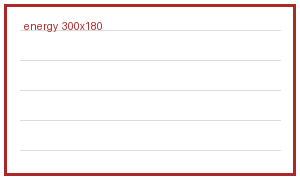
\includegraphics[width=\linewidth]{figures/energy.png}
  \caption{Energy per inference as a function of the accuracy budget.}
  \label{fig:energy}
\end{figure}

\begin{figure}[t]
  \centering
  \includegraphics[width=\linewidth]{figures/ablation.png}
  \caption{Ablation over the truncation schedule.}
  \label{fig:ablation}
\end{figure}

\subsection{Ablation}

Removing the noise floor term ($\eta = 0$) increases the MAC count by 8.4\% at equal
accuracy, confirming that the additive term is not cosmetic. See
Figure~\ref{fig:ablation} for the full sweep.

\section{Discussion}
\label{sec:discussion}

The closed-form rank in Equation~\eqref{eq:rank} assumes that the singular spectrum is
stationary across calibration batches. This holds for the layers we examined but fails
for the first convolutional layer, where the input distribution shifts with the
data augmentation policy. Practitioners should therefore exclude the stem layer from
automatic truncation.

Our results also suggest a limitation: AST is orthogonal to architectural search
\citep{tan2019efficientnet}, and the two were not combined here. This is left for
future work, as discussed in Section~\ref{sec:missing}.

\section{Conclusion}
\label{sec:conclusion}

We presented \method{}, a calibration-time spectral truncation scheme for low-power edge
inference. AST reduces MAC operations by 41.7\% on ResNet-18 with a 0.6 percentage point
accuracy loss, requires no retraining, and composes with post-training quantization.


\section*{Declaration of Competing Interest}
The authors declare that they have no known competing financial interests or personal
relationships that could have appeared to influence the work reported in this paper.

% [sci-trans] 目标期刊强制要求的声明（内容需作者填写）
\section*{Funding}
[待作者填写]
\section*{Data Availability Statement}
[待作者填写]

\bibliographystyle{elsarticle-num}
\bibliography{refs}

\end{document}

\endinput
